% !TEX TS-program = xelatex
\documentclass[10pt,portrait,a4paper]{article}
%\usepackage[utf8]{inputenc}
%\usepackage[ngerman]{babel}
\usepackage{tikz}
\usetikzlibrary{shapes,positioning,arrows,fit,calc,graphs,graphs.standard}
\usepackage[nosf]{kpfonts}
\usepackage[t1]{sourcesanspro}
%\usepackage[lf]{MyriadPro}
%\usepackage[lf,minionint]{MinionPro}
\usepackage{multicol}
\usepackage{wrapfig}
\usepackage[top=0mm,bottom=1mm,left=0mm,right=1mm]{geometry}
\usepackage[framemethod=tikz]{mdframed}
\usepackage{microtype}
%\usepackage{physics}

\newcommand\codeblue[1]{\textcolor{blue}{\code{#1}}}

\usepackage{lastpage}
\usepackage{datetime}
\yyyymmdddate
\renewcommand{\dateseparator}{-}
\let\bar\overline

\definecolor{myblue}{cmyk}{1,.72,0,.38}

\def\firstcircle{(0,0) circle (1.5cm)}
\def\secondcircle{(0:2cm) circle (1.5cm)}

\colorlet{circle edge}{myblue}
\colorlet{circle area}{myblue!5}

\tikzset{filled/.style={fill=circle area, draw=circle edge, thick},
    outline/.style={draw=circle edge, thick}}

\pgfdeclarelayer{background}
\pgfsetlayers{background,main}

\everymath\expandafter{\the\everymath \color{myblue}}
%\everydisplay\expandafter{\the\everydisplay \color{myblue}}


\renewcommand{\baselinestretch}{.8}
\pagestyle{empty}

\global\mdfdefinestyle{header}{%
linecolor=gray,linewidth=1pt,%
leftmargin=0mm,rightmargin=0mm,skipbelow=0mm,skipabove=0mm,
}

\newcommand{\header}{
\begin{mdframed}[style=header]
\footnotesize
\sffamily
CS1101S Finals Cheatsheet v1.2\\(\today)\\
by~indocomsoft,~page~\thepage~of~\pageref{LastPage}
\end{mdframed}
}
%\usepackage{chngcntr}

\usepackage{verbatim}
\counterwithin*{equation}{section}
\counterwithin*{equation}{subsection}
\usepackage{enumitem}
\newlist{legal}{enumerate}{10}
\setlist[legal]{label*=\arabic*.,leftmargin=2.5mm}
\setlist[itemize]{leftmargin=2.5mm}
\setlist{nosep}
\usepackage{minted}

\def\code#1{\texttt{#1}}

\newenvironment{descitemize} % a mixture of description and itemize
{\begin{description}[leftmargin=*,before=\let\makelabel\descitemlabel]}
  {\end{description}}

\newcommand{\descitemlabel}[1]{%
  \textbullet\ \textbf{#1}%
}
\makeatletter



\renewcommand{\section}{\@startsection{section}{1}{0mm}%
                                {.2ex}%
                                {.2ex}%x
                                {\color{myblue}\sffamily\small\bfseries}}
\renewcommand{\subsection}{\@startsection{subsection}{1}{0mm}%
                                {.2ex}%
                                {.2ex}%x
                                {\sffamily\bfseries}}
\renewcommand{\subsubsection}{\@startsection{subsubsection}{1}{0mm}%
                                {.2ex}%
                                {.2ex}%x
                                {\rmfamily\bfseries}}



\def\multi@column@out{%
   \ifnum\outputpenalty <-\@M
   \speci@ls \else
   \ifvoid\colbreak@box\else
     \mult@info\@ne{Re-adding forced
               break(s) for splitting}%
     \setbox\@cclv\vbox{%
        \unvbox\colbreak@box
        \penalty-\@Mv\unvbox\@cclv}%
   \fi
   \splittopskip\topskip
   \splitmaxdepth\maxdepth
   \dimen@\@colroom
   \divide\skip\footins\col@number
   \ifvoid\footins \else
      \leave@mult@footins
   \fi
   \let\ifshr@kingsaved\ifshr@king
   \ifvbox \@kludgeins
     \advance \dimen@ -\ht\@kludgeins
     \ifdim \wd\@kludgeins>\z@
        \shr@nkingtrue
     \fi
   \fi
   \process@cols\mult@gfirstbox{%
%%%%% START CHANGE
\ifnum\count@=\numexpr\mult@rightbox+2\relax
          \setbox\count@\vsplit\@cclv to \dimexpr \dimen@-1cm\relax
\setbox\count@\vbox to \dimen@{\vbox to 1cm{\header}\unvbox\count@\vss}%
\else
      \setbox\count@\vsplit\@cclv to \dimen@
\fi
%%%%% END CHANGE
            \set@keptmarks
            \setbox\count@
                 \vbox to\dimen@
                  {\unvbox\count@
                   \remove@discardable@items
                   \ifshr@nking\vfill\fi}%
           }%
   \setbox\mult@rightbox
       \vsplit\@cclv to\dimen@
   \set@keptmarks
   \setbox\mult@rightbox\vbox to\dimen@
          {\unvbox\mult@rightbox
           \remove@discardable@items
           \ifshr@nking\vfill\fi}%
   \let\ifshr@king\ifshr@kingsaved
   \ifvoid\@cclv \else
       \unvbox\@cclv
       \ifnum\outputpenalty=\@M
       \else
          \penalty\outputpenalty
       \fi
       \ifvoid\footins\else
         \PackageWarning{multicol}%
          {I moved some lines to
           the next page.\MessageBreak
           Footnotes on page
           \thepage\space might be wrong}%
       \fi
       \ifnum \c@tracingmulticols>\thr@@
                    \hrule\allowbreak \fi
   \fi
   \ifx\@empty\kept@firstmark
      \let\firstmark\kept@topmark
      \let\botmark\kept@topmark
   \else
      \let\firstmark\kept@firstmark
      \let\botmark\kept@botmark
   \fi
   \let\topmark\kept@topmark
   \mult@info\tw@
        {Use kept top mark:\MessageBreak
          \meaning\kept@topmark
         \MessageBreak
         Use kept first mark:\MessageBreak
          \meaning\kept@firstmark
        \MessageBreak
         Use kept bot mark:\MessageBreak
          \meaning\kept@botmark
        \MessageBreak
         Produce first mark:\MessageBreak
          \meaning\firstmark
        \MessageBreak
        Produce bot mark:\MessageBreak
          \meaning\botmark
         \@gobbletwo}%
   \setbox\@cclv\vbox{\unvbox\partial@page
                      \page@sofar}%
   \@makecol\@outputpage
     \global\let\kept@topmark\botmark
     \global\let\kept@firstmark\@empty
     \global\let\kept@botmark\@empty
     \mult@info\tw@
        {(Re)Init top mark:\MessageBreak
         \meaning\kept@topmark
         \@gobbletwo}%
   \global\@colroom\@colht
   \global \@mparbottom \z@
   \process@deferreds
   \@whilesw\if@fcolmade\fi{\@outputpage
      \global\@colroom\@colht
      \process@deferreds}%
   \mult@info\@ne
     {Colroom:\MessageBreak
      \the\@colht\space
              after float space removed
              = \the\@colroom \@gobble}%
    \set@mult@vsize \global
  \fi}
\global\let\tikz@ensure@dollar@catcode=\relax
\makeatother
\setlength{\parindent}{0pt}

\setminted{tabsize=2, breaklines}
% Remove belowskip of minted
\setlength\partopsep{-\topsep}

\setlength\columnsep{1.5pt}
\setlength\columnseprule{0.1pt}
\begin{document}
\setlength{\abovedisplayskip}{0pt}
\setlength{\belowdisplayskip}{0pt}

\tiny
\begin{multicols*}{4}
  \raggedcolumns
  \section{Source Week 11 Syntax}
  Two functions/objects may have the same definition, but \codeblue{===} returns \textbf{false} because each function is unique. This includes non-primitives, e.g. \codeblue{[]===[]} returns true.\\
  Note also that passing non-primitives as an argument to a function passes a pointer. (But javascript does not expose changing-pointer-pointing-to-which-memory-address mechanism). So, JS-to-C equivalent:
  \begin{itemize}
    \item \codeblue{fn(arr)}$\equiv$ \codeblue{fn(\&arr)}
    \item Inside \codeblue{fn}: \codeblue{arr[5]} $\equiv$ \codeblue{arr[5]}$\equiv$\codeblue{*(arr+5)}
    \item Hence, inside \codeblue{fn}: \codeblue{ret = []; arr = ret;} does not mutate the original arr as it is just a pointer, but \codeblue{arr[2]=5;} does mutate the original array.
  \end{itemize}
  \subsection*{math\_<name>, where \codeblue{name} can be:}
  \begin{descitemize}
    \item [const:] \codeblue{E, LN10, LN2, LOG10E, LOG2E, PI, SQRT1\_2, SQRT2}
    \item [Functions:] \codeblue{abs(x), cbrt(x), ceil(x), exp(x), floor(x), log(x), log10(x), log2(x), max(x1,...,xn), min(x1,...,xn), pow(base, exponent), random(), round(x), sqrt(x), trunc(x), acos(x), asin(x), atan(x), cos(x), sin(x), tan(x)}
  \end{descitemize}
  \subsection*{General Functions}
  \begin{itemize}
    \begin{minipage}{\columnwidth}
      \setlength\columnseprule{0pt}
      \setlength{\topskip}{0pt}
      \begin{multicols*}{2}
        \item \codeblue{parseInt(string)}
        \item \codeblue{alert(string)}
        \item \codeblue{display(value)}
        \item \codeblue{prompt(string)}
      \end{multicols*}
    \end{minipage}
  \end{itemize}
  \subsection*{Primitive Data Type Checks}
  \begin{itemize}
    \begin{minipage}{\columnwidth}
      \setlength\columnseprule{0pt}
      \setlength{\topskip}{0pt}
      \begin{multicols*}{3}
        \item \codeblue{is\_boolean}
        \item \codeblue{is\_number}
        \item \codeblue{is\_string}
        \item \codeblue{is\_function}
        \item \codeblue{is\_object}
        \item \codeblue{is\_array}
      \end{multicols*}
    \end{minipage}
  \end{itemize}
  PS: \codeblue{is\_object(array)} returns \codeblue{true}x
  \subsection*{List Library}
  \begin{itemize}
    \item \codeblue{pair(x,y)}: Makes a pair from x and y.
    \item \codeblue{head(p)}: Returns the head (first component) of the pair x.
    \item \codeblue{tail(p)}: Returns the tail (second component) of the pair x.
    \item \codeblue{set\_head(p,x)}: Sets the head (first component) of the pair p to be x; returns undefined.
    \item \codeblue{set\_tail(p,x)}: Sets the tail (second component) of the pair p to be x; returns undefined.
    \item \codeblue{list(x1,x2,...,xn)}: Returns a list with n elements. The first element is x1, the second x2, etc. Iterative process; time: $O(n)$, space: $O(n)$, since the constructed list data structure consists of n pairs, each of which takes up a constant amount of space.
    \item \codeblue{is\_pair(p)}: Returns true if x is a pair and false otherwise.
    \item \codeblue{is\_empty\_list(x)}: Returns true if xs is the empty list, and false otherwise.
    \item \codeblue{is\_list(x)}: Returns true if x is a list as defined in the lectures, and false otherwise. Iterative process; time: O(n), space: O(1), where n is the length of the chain of tail operations that can be applied to x.
    \item \codeblue{length(xs)}: Returns the length of the list xs. Iterative process; time: O(n), space: O(1), where n is the length of xs.
    \item \codeblue{map(f,xs)}: Returns the length of the list xs. Iterative process; time: O(n), space: O(1), where n is the length of xs.
    \item \codeblue{build\_list(n,f)}: Makes a list with n elements by applying the unary function f to the numbers 0 to n - 1. Recursive process; time: O(n), space: O(n).
    \item \codeblue{for\_each(f,xs)}: Applies f to every element of the list xs, and then returns true. Iterative process; time: O(n), space: O(1), where n is the length of xs
    \item \codeblue{list\_to\_string(xs)}: Returns a string that represents list xs using the text-based box-and-pointer notation [...].
    \item \codeblue{reverse(xs)}: Returns list xs in reverse order. Iterative process; time: O(n), space: O(n), where n is the length of xs. The process is iterative, but consumes space O(n) because of the result list.
    \item \codeblue{append(xs,ys)}: Returns a list that results from appending the list ys to the list xs. Recursive process; time: O(n), space: O(n), where n is the length of xs.
    \item \codeblue{member(x,xs)}: Returns first postfix sublist whose head is identical to x (===); returns [] if the element does not occur in the list. Iterative process; time: O(n), space: O(1), where n is the length of xs.
    \item \codeblue{remove(x,xs)}: Returns a list that results from xs by removing the first item from xs that is identical (===) to x. Recursive process; time: O(n), space: O(n), where n is the length of xs.
    \item \codeblue{remove\_all(x)}:Returns a list that results from xs by removing all items from xs that are identical (===) to x. Recursive process; time: O(n), space: O(n), where n is the length of xs.
    \item \codeblue{filter(pred,xs)}: Returns a list that contains only those elements for which the one-argument function pred returns true. Recursive process; time: O(n), space: O(n), where n
          is the length of xs.
    \item \codeblue{enum\_list(start,end)}: Returns a list that enumerates numbers starting from start using a step size of 1, until the number exceeds (>) end. Recursive process; time: O(n), space: O(n), where n is the length of xs.
    \item \codeblue{list\_ref(xs,n)}: Returns the element of list xs at position n, where the first element has index 0. Iterative process; time: O(n), space: O(1), where n is the length of xs.
    \item \codeblue{accumulate(op,initial,xs)}: Applies binary function op to the elements of xs from right-to-left order, first applying op to the last element and the value initial, resulting in r1, then to the second-last element and r1, resulting in r2, etc, and finally to the first element and rn-1, where n is the length of the list. Thus, accumulate(op,zero,list(1,2,3)) results in op(1, op(2, op(3, zero))). Recursive process; time: O(n), space: O(n), where n is the length of xs, assuming op takes constant time.
  \end{itemize}
  \subsection*{Misc Functions}
  \begin{itemize}
    \item \codeblue{equal(x, y)} - \codeblue{true} if pairs and corrs leaves are \codeblue{===}
    \item \codeblue{array\_length(arr)} $=1+$(highest index used)
    \item \codeblue{apply\_in\_underlying\_javascript(f, xs)}:\\ calls the function f with arguments xs. For example:\\
          \begin{minipage}{\columnwidth}
            \begin{minted}{javascript}
function times(x, y) {
  return x * y;
}
apply_in_underlying_javascript(times, list(2, 3));
// returns 6
          \end{minted}
          \end{minipage}

  \end{itemize}

  \subsection*{OOP Inheritance, method declaration, constructor example code}
  \begin{minted}{javascript}
function icsbot(name){ Player.call(this, name); }
icsbot.Inherits(Player);
icsbot.prototype.__act = function(){
  Player.prototype.__act.call(this);
  ...
}
var anu = new Player("abc");
\end{minted}
  \subsection*{OOP Syntactic Sugar}
  \begin{descitemize}
    \item \codeblue{Object.attribute = 5;} =>\\
    \begin{minipage}{\columnwidth}
      \begin{minted}{javascript}
Object["attribute"] = 5;
    \end{minted}
    \end{minipage}
    \item \codeblue{Object.method(arg1, arg2, ...)} =>\\
    \begin{minipage}{\columnwidth}
      \begin{minted}{javascript}
var newid = object;
newid["method"].call(newid, arg1, arg2, ...);
\end{minted}
    \end{minipage}
    \item \codeblue{ChildClass.Inherits(ParentClass)} => \\
    \begin{minipage}{\columnwidth}
      \begin{minted}{javascript}
ChildClass.prototype.__proto__=ParentClass.prototype;
  \end{minted}
    \end{minipage}
    \item \codeblue{var anu = new Player("abc");} => \\
    \begin{minipage}{\columnwidth}
      \begin{minted}{javascript}
var anu = {};
anu.prototype.__proto__ = Player.prototype;
Player.call(anu, "abc");
  \end{minted}
    \end{minipage}
  \end{descitemize}
  \section{Complexity}
  \begin{descitemize}
    \item [Big Oh $O()$]: Upper bound (worst case)
    \item [Big Omega $\Omega()$]: Lower bound (best case)
    \item [Big Theta $\Theta()$]: Both upper and lower bound
    \item [Order]:\\
    $\Theta(1) < \Theta(\log n) < \Theta(n) < \Theta(n \log n) < \Theta(n^2) < \Theta(n^3) < \Theta(2^n) < \Theta(3^n) < \Theta(n^n)$
  \end{descitemize}

  \section{Box-and-Pointer Diagrams}
  \begin{minted}{javascript}
var w1 = list(1,2); var w2 = list(3,4);
var w3 = append(w1,w2);
\end{minted}
  \begin{verbatim}
    +---+   +---+
w1->|1| |-->|2|/|
    +---+   +---+
w2-------------------+
                     v
    +---+   +---+   +---+   +---+
w3->|1| |-->|2| |-->|3| |-->|4|/|
    +---+   +---+   +---+   +---+
\end{verbatim}
  \begin{minted}{javascript}
var x = list(pair(1,2), pair(3,4));
set_tail(head(x), head(tail(x)));
\end{minted}
  \begin{verbatim}
   +---+   +---+
x->| | |-->| |/|
   +---+   +---+
    V       V
   +---+   +---+
   |1| |-->|3|4|
   +---+   +---+
\end{verbatim}
  \begin{minted}{javascript}
var input = list(1, pair(2,3), list(4));
var result = map(function(x){return x;}, input);
\end{minted}
  \begin{verbatim}
        +---+   +---+   +---+
input-->|1| |-->| | |-->| |/|
        +---+   +---+   +---+
                 V       V
                +---+   +---+
                |2|3|   |4|/|
                +---+   +---+
                 ^       ^
        +---+   +---+   +---+
result->|1| |-->| | |-->| |/|
        +---+   +---+   +---+
\end{verbatim}

  \section{List-related}
  \subsection*{contains}
  \begin{minted}{javascript}
function contains(x, xs) {
    return !is_empty_list(member(x, xs));
}
\end{minted}
  \subsection*{Map}
  \begin{minted}{javascript}
function map(f, xs) {
  return is_empty_list(xs)
            ? []
            : pair(f(head(xs)), map(f, tail(xs)));
}
// iterative alternative
function new_map(f, xs) {
  function helper(xs, acc) {
    return is_empty_list(xs)
            ? acc
            : helper(tail(xs), pair(f(head(xs)), acc));
  }
  return reverse(helper(xs, []));
}
\end{minted}
  \subsection*{Filter}
  \begin{minted}{javascript}
function filter(pred, xs) {
  if(is_empty_list(xs)) {
    return [];
  } else {
    return pred(head(x))
            ? pair(head(xs), filter(pred, tail(xs)))
            : filter(pred, tail(xs));
  }
}
// filter with accumulate
function new_filter(pred, xs) {
  return accumulate(function(e, acc){
                      return pred(e) ? pair(e, acc)
                                     : acc;
                    }, [], xs);
}
\end{minted}
  \subsection*{Reverse}
  \begin{minted}{javascript}
function reverse(xs) {
  function rev(original, reversed) {
    return is_empty_list(original)
            ? reversed
            : rev(tail(original), pair(head(original), reversed));
  }
  return rev(xs,[]);
}
function reverse(lst) {
  return append(reverse(tail(lst)), list(head(lst)));
}
\end{minted}
  \subsection*{next\_nth, every\_n}
  \begin{minted}{javascript}
// every_n returns every n-th element from lst
function next_nth(lst, n) {
  if (is_empty_list(lst)) {
    return [];
  } else if (n === 1) {
    return lst;
  } else {
    return next_nth(tail(lst), n - 1);
  }
}
function every_n(lst, n) {
  var next_element = next_nth(lst, n);
  if (is_empty_list(next_element)) {
    return [];
  } else {
    return pair(head(next_element),
                every_n(tail(next_element), n));
  }
}
function find(v, xs){
  return (is_empty_list(xs)) ? false
            : (v === head(xs)) ? true
                               : find(v, tail(xs));
}
  \end{minted}
  \subsection*{Deep Copy}
  \begin{minted}{javascript}
function deep_copy(xs) {
  return map(function(x) {
               return is_number(x) ? x : deep_copy(x);
             }, xs);
}
  \end{minted}
  \subsection*{Variations of accumulate}
  \begin{minted}{javascript}
//accumulate_n(list(list(1,2,3),list(4,5,6),list(7,8,9)), 0, s) = list(12,15,18)
function accumulate_n(op, init, seqs) {
  if (is_empty_list(head(seqs))) {
    return [];
  } else {
    return pair(accumulate(op, init,
                   map(function(x){ return head(x); }, seqs)),
                accumulate_n(op, init,
                   map(function(x){ return tail(x); }, seqs)));
  }
}
//accumulate_tree(plus,0,list(1,2,list(3,4), list(5,list(6,7)))) = 28
function accumulate_tree(op, initial, seq) {
  return accumulate(
            function(a, b){
               return a + (is_list(b) ? accumulate_tree(op, initial, b) : b);
            }, initial, seq);
}
var fold_right = accumulate;
function fold_left(op, initial, sequence) {
  function iter(result, rest) {
     return is_empty_list(rest)
              ? result
              : iter(op(result, head(rest)), tail(rest));
  }
  return iter(initial, sequence);
}
  \end{minted}
  \subsection*{Count Pairs}
  \begin{minted}{javascript}
function count_pairs(x) {
  var hist = [];
  function helper(x) {
    if(!is_pair(x)) {
      return 0;
    } else {
      if(is_empty_list(member(x, hist))) {
        hist = pair(x, hist);
        return 1 + helper(head(x)) + helper(tail(x));
      } else {
        return 0;
      }
    }
  }
  return helper(x);
}
\end{minted}
  \section{Higher Order Function}
  \subsection*{Compose, Identity}
  \begin{minted}{javascript}
function compose(f, g){
  return function(x){ return f(g(x)); };
}
function identity(x) {
  return x;
}
function repeated(f, n) {
  return (n === 0) ? identity : compose(f, repeated(f, n - 1));
}

function plus_one (x) {
  return x + 1;
}
function twice (f) {
  return function(x) { return f(f(x)); };
}
\end{minted}
  Evaluate:\codeblue{(twice(twice(twice)))(twice)(plus\_one)(4)}
  \begin{equation*}
    t^{2^{((2^2)^2)}}=t^{2^{(4)^2}}=t^{2^{16}}=t^{65536}
  \end{equation*}
  \codeblue{twice} does tetration (right-to-left).
  \subsection*{Sum}
  \begin{minted}{javascript}
//Sum: term - the operator, next - (de/in)crement counter, a - starting point, b - endpoint
// recursive version
function sum(term, a, next, b) {
  return a > b ? 0 : term(a) + sum(term, next(a), next, b);
}
// iterative version
function sum(term, a, next, b) {
  function sum_iter(x, total) {
    return x > b ? total : sum_iter(next(x), total + term(x));
  }
  return sum_iter(a, 0);
}
  \end{minted}
  \section{Data Structures}
  \subsection*{Queue \textmd{(enqueue in $O(n)$, the rest in $O(1)$)}}
  \begin{minted}{javascript}
function empty_queue() { return []; }
function enqueue(x, q) {
  return is_empty_list(q)
          ? pair(x, empty_queue());
          : pair(head(q), enqueue(x, tail(q)));
  }
}
function dequeue(x, q){ return tail(q); }
function qhead(q){ return head(q); }
  \end{minted}
  \subsection*{Trees}
  \begin{minted}{javascript}
function count_data_items(tree) {
  return is_empty_list(tree)
            ? 0
            : (is_list(head(tree))
                ? count_data_items(head(tree))
                : 1)
          + count_data_items(tail(tree));
}
function map_tree(f, tree) {
  return map(function(sub_tree) {
              return !is_list(sub_tree) ? f(sub_tree) : map_tree(f,sub_tree);
             }, tree);
}
function accumulate_tree(f, init, xs) {
  return accumulate(function(e, acc) {
                      return (is_list(e))
                        ? f(accumulate_tree(f, init, e), acc)
                        : f(e, acc);
                    }, init, xs);
}
function is_number_tree(xs) {
  if (!is_list(xs)) { return false;
  } else {
    return accumulate(function(e, acc){
                        return acc && (is_list(e)
                                    ? is_number_tree(e)
                                    : is_number(e));
                      }, true, xs);
  }
}
  \end{minted}
  \subsection*{Balanced BST}
  \begin{minted}{javascript}
function make_node(left_tree, number, right_tree) {
  return list(left_tree, number, right_tree);
}
function middle(n) { return math_floor(n / 2); }
function take(xs, n) {
  return n === 0 ? [] : pair(head(xs), take(tail(xs), n - 1));
}
function drop(xs, n) {
  return n === 0 ? xs : drop(tail(xs), n - 1);
}
function make_balanced(xs) {
  var list_length = length(xs);
  if (list_length === 0) {
    return [];
  } else {
    var list_mid = middle(list_length);
    return make_node(make_balanced(take(xs, list_mid)),
                     list_ref(xs, list_mid),
                     make_balanced(drop(xs, list_mid + 1)));
  }
}
\end{minted}
  \section{Mutable Data Structure}
  \subsection*{Tortoise and Hare Algorithm (check if list has a loop)}
  \begin{minted}{javascript}
function has_loop(lst) {
  function tortoise_and_hare(tortoise, hare) {
    if (is_empty_list(tortoise) || is_empty_list(hare) || is_empty_list(tail(hare))) {
      return false;
    } else {
      return tortoise === hare
              ? true
              : tortoise_and_hare(tail(tortoise), tail(tail(hare)));
    }
  }
  return tortoise_and_hare(lst, tail(lst));
}
\end{minted}
  \subsection*{Circular List}
  \begin{minted}{javascript}
function make_circular_copy(xs) {
  function inner(zs, ys) {
    if (is_empty_list(zs)) {
      return ys;
    } else {
      return pair(head(zs), inner(tail(zs), ys));
    }
  }
  if (is_empty_list(xs)) {
    return [];
  } else {
    var ys = pair(head(xs), []);
    set_tail(ys, inner(tail(xs), ys));
    return ys;
  }
}
function make_linear(xs) {
  function helper(lst) {
    if (tail(lst) === xs) {
      set_tail(lst, []);
    } else {
      helper(tail(lst));
    }x
  }
}
\end{minted}
  \subsection*{Queue in $O(1)$ using mutable data structure}
  \begin{minted}{javascript}
// Queue data structure
function make_queue() { return pair([], []); }
function is_empty_queue(q) {
    return is_empty_list(head(q));
}
function enqueue(q, item) {
    if (is_empty_queue(q)) {
        set_head(q, pair(item, []));
        set_tail(q, head(q));
    } else {
        set_tail(tail(q), pair(item, []));
        set_tail(q, tail(tail(q)));
    }
}
function dequeue(q) {
    var front = head(head(q));
    set_head(q, tail(head(q)));
    return front;
}
function peek(q) { return head(head(q)); }
  \end{minted}
  \subsection*{Stack}
  \begin{minted}{javascript}
function make_stack() { return pair("stack", []); }
function is_empty_stack(stack) {
  return is_empty_list(tail(stack));
}
function peek(stack) {
  return is_empty_stack(stack) ? "stack underflow"
                               : head(tail(stack));
}
function push(stack, x) {
    set_tail(stack, pair(x, tail(stack)));
}
function pop(stack) {
    if (is_empty(stack)) {
        return "stack underflow";
    } else {
        var top = peek(stack);
        set_tail(stack, tail(tail(stack)));
        return top;
    }
}
\end{minted}
  \subsection*{Mutable version of list functions}
  \begin{minted}{javascript}
function mutable_append(xs, ys) {
  if (is_empty_list(xs)) {
    return ys;
  } else {
    set_tail(xs, mutable_append(tail(xs), ys));
    return xs;
  }
}

function mutable_reverse(xs) {
  function help(ori, rev) {
    if (is_empty_list(ori)) {
      return rev;
    } else {
      var temp = tail(ori);
      set_tail(ori, rev);
      return help(temp, ori);
    }
  }
}
\end{minted}
  \section{Coin Change}
  \begin{minted}{javascript}
// cc(25, list(5, 10, 20, 50, 100));
function cc(amount, lst) {
  var coins = pair(0, lst);
  function helper(amount, coin_range) {
    if (amount === 0) { return 1;
    } else if (amount < 0 || coin_range === 0) {
      return 0;
    } else {
      return helper(amount, coin_range - 1)
             + helper(amount - list_ref(coins, coin_range), coin_range);
    }
  }
  return helper(amount, length(lst));
}
// Given coins in list l, return list of coin permutations that add up to x
function makeup_amount(x,l) {
  if (is_pair(l)) {
    return append(map(function(x){ return pair(head(l),x); },
                      makeup_amount(x - head(l), tail(l))),
                  makeup_amount(x, tail(l)));
  } else if (x === 0) {
      return list([]);
  } else {
      return [];
  }
}
  \end{minted}
  \subsection*{Doubly-linked List}
  \begin{minted}{javascript}
function make_node(data, prev, next) {
  return list("node", data, prev, next);
}
function get_prev(node) {
  return head(tail(tail(node)));
}
function get_next(node) {
  return head(tail(tail(tail(node))));
}
function get_data(node) { return head(tail(node)); }
function empty_node() { return make_node([], [], []); }
function is_empty_node(node) {
    return head(node) === "node" && equal(node, empty_node());
}
function set_data(n, v) {
    var temp = list(v, get_prev(n), get_next(n));
    set_tail(n, temp);
}
function set_previous(n, v) {
    var temp = list(get_data(n), v, get_next(n));
    set_tail(n, temp);
}
function set_next(n, v) {
    var temp = list(get_data(n), get_prev(n), v);
    set_tail(n, temp);
}
function insert_before(n1, n2) {
    set_prev(n2, get_prev(n1));
    set_next(get_prev(n1), n2);
    set_prev(n1, n2); set_next(n2, n1);
}
function insert_after(n1, n2) {
  set_next(n2, get_next(n1));
  set_prev(get_next(n1), n2);
  set_next(n1, n2); set_prev(n2, n1);
}
function remove(n) {
  var x = get_prev(n); var y = get_next(n);
  set_next(x, y); set_prev(y, x);
}
function dlist_to_list(dlst) {
  return is_empty_node(dlst)
          ? []
          : pair(get_data(dlst), dlist_to_list(get_next(dlst)));
}
function list_to_dlist(lst) {
  var first_node = make_node(head(lst), empty_node(), empty_node());
  var prev_node = first_node;
  for_each(function(x){
             var new_node = make_node(x, prev_node, empty_node());
             set_next(prev_node, new_node);
             prev_node = new_node;
           }, tail(lst));
  return first_node;
}
function reverse_dlist(dlst) {
  return list_to_dlist(reverse(dlist_to_list(dlst)));
}
\end{minted}
  \section{Permutations \& Combinations}
  \subsection*{Permutations \textmd{($O(n!)$)} and permutations\_r \textmd{($O\left(\frac{n!}{(n-r)!}\right)$)}}
  \begin{minted}{javascript}
function permutations(s) {
  if (is_empty_list(s)) {
      return list([]);
  } else {
      return accumulate(append, [], map(function(x) {
               return map(function(p) {
                            return pair(x, p);
                          }, permutations(remove(x, s)));
                    }, s));
  }
}
function permutations_r(s, r) {
  if (r === 0) { return list([]);
  } else if(is_empty_list(s)){ return list();
  } else {
    return accumulate(append, [], map(function(x) {
            return map(function(p) {
                         return pair(x, p);
                       }, permutations_r(remove(x, s), r - 1));
                  }, s));
  }
}
  \end{minted}
  \subsection*{Combinations \textmd{($O\left(\frac{n!}{(n-k)!k!}\right) = O\left(n^{n\div 2}\right)$)}}
  \begin{minted}{javascript}
function combinations_k(xs, k) {
  if (k === 0) { return list([]);
  } else if (is_empty_list(xs)) { return [];
  } else {
    var s1 = combinations(tail(xs), k - 1);
    var s2 = combinations(tail(xs), k);
    var x = head(xs);
    var has_x = map(function(s) { return pair(x, s);}, s1);
    return append(has_x, s2);
  }
}
    \end{minted}
  \subsection*{Power Set}
  \begin{minted}{javascript}
function power_set(xs) {
  if (is_empty_list(xs)) {
    return list([]);
  } else {
    // Either you pick the number, or you don't
    var without_head=power_set(tail(xs));
    var use_head = map(function(l) {
                         return pair(head(xs),l);
                       }, without_head);
    return append(use_head,without_head);
  }
}
function are_equal_sets(set1, set2) {
  if(length(set1) === length(set2)) {
    return false;
  } else {
    return accumulate(function(e1,acc){
              return accumulate(function(e2,acc) {
                      return e2 === e1 || acc;
              }, false, set2);
            }, true, set1);
  }
}
  \end{minted}
  \section{Tower of Hanoi}
  \subsection*{Tower of Hanoi \textmd{(Running time: $O(2^n)$)}}
  \begin{minted}{javascript}
function make_move(from, to) { return list(from, to); }
function hanoi(n, A, B, C) {
  if (n === 1) { return list(make_move(A, B));
  } else {
    var moves_to_helper = hanoi(n - 1, A, C, B);
    var the_move = make_move(A, B);
    var moves_to_final = hanoi(n - 1, C, B, A);
    return append(moves_to_helper, pair(the_move, moves_to_final));
  }
}
  \end{minted}
  \section{Sorting functions \& Binary Search}
  \subsection*{Selection Sort \textmd{($\Theta(n^2)$)}}
  \begin{minted}{javascript}
  function selection_sort(xs) {
    if (is_empty_list(xs)) { return xs;
    } else {
      var x = smallest(xs);
      return pair(x, selection_sort(remove(x, xs)));
    }
  }
  // find smallest element of a non-empty list xs
  function smallest(xs) {
    function sm(x, ys) {
      return is_empty_list(ys)
              ? x
              : x < head(ys) ? sm(x, tail(ys))
                             : sm(head(ys), tail(ys));
    }
    return sm(head(xs), tail(xs));
  }
    \end{minted}
  \subsection*{Insertion Sort \textmd{(Input-dependent, best:$\Omega(n)$, worst:$O(n^2)$)}}
  \begin{minted}{javascript}
function insert(x, xs) {
  return is_empty_list(xs)
           ? list(x)
           : x <= head(xs) ? pair(x,xs)
                           : pair(head(xs), insert(x,tail(xs)));
}
function insertion_sort(xs) {
  return is_empty_list(xs) ? xs : insert(head(xs),insertion_sort(tail(xs)));
}
  \end{minted}
  \subsection*{Merge Sort \textmd{(Running time: $\Theta(n \log n)$)}}
  \begin{minted}{javascript}
function middle(n) { return math_floor(n / 2); }
function take(xs, n) {
    return n === 0 ? []
                   : pair(head(xs),take(tail(xs),n-1));
}
function drop(xs, n) {
    return n === 0 ? xs : drop(tail(xs), n - 1);
}
function merge(xs, ys) {
    if (is_empty_list(xs)) { return ys;
    } else if (is_empty_list(ys)) { return xs;
    } else {
        var x = head(xs); var y = head(ys);
        return (x < y) ? pair(x, merge(tail(xs), ys))
                       : pair(y, merge(xs, tail(ys)));
    }
}
function merge_sort(xs) {
    if (is_empty_list(xs) || is_empty_list(tail(xs))) {
        return xs;
    } else {
        var mid = middle(length(xs));
        return merge(merge_sort(take(xs, mid)),
                     merge_sort(drop(xs, mid)));
    }
}
  \end{minted}
  \subsection*{Quicksort \textmd{(Input-dependent, best: $\Omega(n \log n)$, worst: $O(n^2)$)}}
  \begin{minted}{javascript}
function partition(xs, p) {
  function helper(lst, smaller, larger) {
    if (is_empty_list(lst)) {
      return pair(smaller, larger);
    } else {
      var cur = head(lst);
      return cur <= p
              ? helper(tail(lst), pair(cur, smaller), larger)
              : helper(tail(lst), smaller, pair(cur, larger));
    }
  }
  return helper(xs, [], []);
}
function quicksort(xs) {
  if (is_empty_list(xs)) { return xs;
  } else if (is_empty_list(tail(xs))) { return xs;
  } else {
    var cur = head(xs);
    var partitioned = partition(tail(xs), cur);
    var sorted_smaller = quicksort(head(partitioned));
    var sorted_larger = quicksort(tail(partitioned));
    return append(sorted_smaller, pair(cur, sorted_larger));
  }
}
  \end{minted}
  \subsection*{Binary Search \textmd{($O(\log n)$), returns true/false}}
  \begin{minted}{javascript}
function binary_search(a, v) {
  function search(low, high) {
    if (low > high) {
      return false;
    } else {
      var mid = math_floor((low + high) / 2);
      return (v === a[mid])
             || (v < a[mid]) ? search(low, mid - 1)
                             : search(mid + 1, high);
    }
  }
  return search(0, array_length(a) - 1);
}
\end{minted}

  \subsection*{Binary Search on sorted rotated array, \textmd{($O(\log n)$), returns the index if found, -1 if not found}}
  \begin{minted}{javascript}
function find(target, arr) {
  function findPivot(low, high) {
    if (low > high) {
      return -1;
    } else {
      var mid = math_floor((low + high) / 2);
      if (mid < high && arr[mid] > arr[mid + 1]) {
        return mid;
      } else if (mid>low && arr[mid] < arr[mid - 1]) {
        return mid - 1;
      } else if (arr[mid] > arr[low]) {
        return findPivot(mid + 1, high);
      } else {
        return findPivot(low, mid - 1);
      }
    }
  }
  function search(low, high) {
    if (low > high) {
      return -1;
    } else {
      var mid = math_floor((low + high) / 2);
      if (target === arr[mid]) {
        return mid;
      } else {
        return target < arr[mid]
                ? search(low, mid - 1)
                : search(mid + 1, high);
      }
    }
  }
  var len = array_length(arr);
  var pivot = findPivot(0, len - 1);
  if (pivot === -1) {
    return search(0, len - 1);
  } else if (arr[0] > target) {
    return search(pivot+1, len - 1);
  } else {
    return search(0, pivot);
  }
}
\end{minted}
  \section{Functions of questionable usefulness}
  \subsection*{DG Week 3}
  \begin{minted}{javascript}
function sum_squares_two_larger(a, b, c){
  return a > b ? a * a + ((b > c) ? b * b : c * c)
               : b * b + ((a > c) ? a * a : b * b)
}
function is_leap_year(year){
    return (year % 4 === 0 && year % 100 !== 0) || year % 400 === 0;
}
  \end{minted}
  \subsection*{DG Week 4}
  \begin{minted}{javascript}
// Pascal Triangle
function pascal(row, column){
  if(column === 1 || row === column){ return 1;
  } else {
      return pascal(row - 1, column - 1) + pascal(row - 1, column);
  }
}
// Additional
function addition(a,n){return repeated(add_one,n)(a);}
function multiplication(a,n){
  var addition_a = function(x){return addition(a,x);};
  return repeated(addition_a,n)(0);
}
function exponentiation(a,n){
  var mul_a = function(x){return multiplication(a,x);};
  return repeated(mul_a,n)(1);
}
function tetration(a,n){
  var exp_a = function(x){return exponentiation(a,x);};
  return repeated(exp_a,n)(1);
}
  \end{minted}
  \section{Functions from Past Year Papers}
  \begin{minted}{javascript}
function is_tree_of_numbers(x) {
  // Solution 1 [5 marks]
  return is_list(x)
         && accumulate(function(a,b){
                         return (is_number(a) || is_tree_of_numbers(a)) && b;
                       }, true, x);
  // Solution 2 [3 marks]
  if (is_empty_list(x)) { return true;
  } else if (is_pair(x)) {
    return (is_number(head(x)) || is_tree_of_numbers(head(x))) && is_tree_of_numbers(tail(x));
  } else { return false;
  }
}
function my_filter(pred, xs) {
  return accumulate(function(a, b) {
                      return pred(a) ? pair(a, b) : b;
                    }, [], xs);
}
  \end{minted}

  \subsection*{2048}
  \begin{minipage}{\columnwidth}
    \begin{minted}{javascript}
function slideRowToTheLeft(arr) {
  for (var i = 0; i < 4; i = i + 1) {
    for (var j = i + 1; j < 4 ; j = j + 1) {
      if (arr[i]===arr[j] && arr[i]!==0 && arr[j] !== 0) {
        arr[i] = 2 * arr[i];
        arr[j]=0;
        break;
      } else { }
    }
  }
  var n = -1;
  for(i = 0; i < 4; i = i + 1) {
    if (arr[i]===0 && n === -1) {
      n = i;
    } else if (arr[i]!== 0 && n > -1) {
      arr[n]=arr[i];
      arr[i]=0;
      i=n;
      n=-1;
    } else { }
  }
  return arr;
}
function slideLeft(grid) {
  for(var i = 0; i < 4; i = i + 1) {
    slideRowToTheLeft(grid[i]);
  }
  return grid;
}

function rotateLeft(grid) {
  var ret = [];
  for(var i = 0; i < 4; i = i + 1) {
    ret[i]=[];
  }
  for(var i=0; i < 4; i = i + 1) {
    for(var j=0; j < 4; j = j + 1) {
      ret[3-j][i]=grid[i][j];
    }
  }
  return ret;
}
function performSlide(grid, direction) {
  if (direction === "left") {
    return slideLeft(grid);
  } else if (direction === "up") {
    return rotateLeft(rotateLeft(rotateLeft(
           slideLeft(rotateLeft(grid)))));
  } else if (direction === "right") {
    return rotateLeft(rotateLeft(slideLeft(rotateLeft(
           rotateLeft(grid)))));
  } else  {
    return rotateLeft(slideLeft(rotateLeft(rotateLeft(
           rotateLeft(grid)))));
  }
}
  \end{minted}
  \end{minipage}
  \section{Memoization}
  \subsection*{1D Memoization Abstraction}
  \begin{minted}{javascript}
function memoize(f) {
  var mem = [];
  return function(x) {
    if (mem[x] !== undefined) { return mem[x];
    } else {
      var result = f(x);
      mem[x] = result;
      return result;
    }
  };
}
// example
var fib=memoize(function(n){
  return n <= 1 ? n : fib(n-1) + fib(n-2);
});
\end{minted}
  \subsection*{Memoized Coin Change}
  \begin{minted}{javascript}
var mem = [];
function read(amount, coin_range) {
  return (mem[amount] === undefined) ? undefined : mem[amount][coin_range];
}
function write(amount, coin_range, value) {
  if (mem[amount] === undefined) {
    mem[amount] = [];
  } else {}
  mem[amount][coin_range] = value;
}
function cc(amount, coin_range) {
  if (read(amount, coin_range) !== undefined) {
    return read(amount, coin_range);
  } else {
    var result = amount === 0 ? 1
                 : (amount < 0 || range === 0) ? 0
                   : cc(amount, range - 1) + cc(amount - highest(range), coin_range);
    write(amount, coin_range, result);
    return result;
  }
}
\end{minted}
  \subsection*{Multi-dimensional Memoization (e.g. Tower of Hanoi)}
  \begin{minted}{javascript}
var mem = [];
function read(w, x, y, z) {
  return (mem[w] === undefined) ? undefined
          : (mem[w][x] === undefined) ? undefined
            : (mem[w][x][y] === undefined) ? undefined : mem[w][x][y][z];
}
function write(w, x, y, z, value) {
  if (mem[w] === undefined) { mem[w] = [];
  } else {}
  if (mem[w][x] === undefined) { mem[w][x] = [];
  } else {}
  if (mem[w][x][y] === undefined) { mem[w][x][y] = [];
  } else {}
  mem[w][x][y][z] = value;
}
function make_move(From, To) { return list(From, To); }
function retriever(n, A, B, C) {
  var result = read(n, A, B, C);
  if (result === undefined) {
    result = mhanoi(n, A, B, C);
    write(n, A, B, C, result);
  } else { }
  return result;
}
function mhanoi(n, A, B, C) {
  var result = retriever(n, A, B, C);
  if (result !== undefined) { return result;
  } else {
    if (n === 1) { return list(make_move(A, B));
    } else {
      var moves_to_helper = retriever(n - 1, A, C, B);
      var the_move = make_move(A, B);
      var moves_to_final = retriever(n - 1, C, B, A);
      return append(moves_to_helper,
                    pair(the_move, moves_to_final));
    }
  }
}
// mhanoi(8, 1, 2, 3);
\end{minted}
  \subsection*{Variation of Knapsack Problem}
  A thief has a getaway car that can hold at most m kg (m is an integer). Write a program that takes in a list of the gold bar masses and determines the total mass of gold bars he can steal. Time complexity:\\
  \textbf{Non-Memoized}: $O(2^{\texttt{length(bar\_masses)}})$,\\
  \textbf{Memoized}: $O(\texttt{length(bar\_masses)}\cdot m)$
  \begin{minted}{javascript}
// Non-memoized version
function max_loot_mass(bar_masses, m) {
  if(is_empty_list(bar_masses)||head(bar_masses) > m) {
    return 0;
  } else {
    var cur = head(bar_masses);
    // Either take the current bar or not
    return math_max(cur + max_loot_mass(tail(bar_masses), m - cur),
                    max_loot_mass(tail(bar_masses), m));
  }
}
// Memoized version
function max_loot_mass(bar_masses, m) {
  var mem = [];
  function write(len, m, value) {
    if (mem[len] === undefined) {
      mem[len] = [];
    } else { }
    countw = countw + 1;
    mem[len][m] = value;
  }
  function read(len, m) {
    if (mem[len] === undefined) { mem[len] = [];
    } else { countr = countr + 1;
    }
    return mem[len][m];
  }
  function helper(bar_masses, m) {
    if (is_empty_list(bar_masses) || head(bar_masses) > m) {
      return 0;
    } else {
      var cur = head(bar_masses);
      var len = length(bar_masses);
      var res = read(len, m);
      if (res === undefined) {
          res = math_max(cur + helper(tail(bar_masses), m - cur), helper(tail(bar_masses), m));
          write(len, m, res);
      } else { }
      return res;
    }
  }
  return helper(bar_masses, m);
}
\end{minted}

  \subsection*{Knapsack Problem: Herbert the Clown}
  Most expensive combination with a given budget from a list of ingredients.\\
  \codeblue{b} = Budget\\
  \codeblue{i\_l} = List of Ingredients Price List\\
  \begin{minipage}{\columnwidth}
    \begin{minted}{javascript}
// Assume all sublists are sorted in ascending order
function getMaxSpend(b, i_l) {
  function is_sufficient_fund(b, i_l) {
    return is_empty_list(i_l)
            ? b >= 0
            :  is_sufficient_fund(b - head(head(i_l)), tail(i_l));
  }
  if (is_sufficient_fund(b, i_l)) {
      if (is_empty_list(i_l) || is_empty_list(head(i_l)) || head(head(i_l)) > b) {
      return 0;
    } else {
      var cur = head(head(i_l));
      var x = cur + getMaxSpend(b - cur, tail(i_l));
      var y = getMaxSpend(b, pair(tail(head(i_l)), tail(i_l)));
      return math_max(x, y);
    }
  } else {
    return -1;
  }
}
var i_l = list(list(4,6,8), list(5,10), list(1,3,5,5));
getMaxSpend(11, i_l); // returns 10 (4+5+1)
getMaxSpend(20, i_l); // returns 19 (8+10+1)

\end{minted}
  \end{minipage}
  \section{Environment Model}
  \begin{minipage}{\columnwidth}
    \setlength{\topskip}{0pt}
    \begin{multicols*}{2}
      \begin{minted}{javascript}
var x = 4;
function foo(x) {
  var y = x * 2;
  if(y===10) {
    x = x + 5;
    return x;
  } else {
    return foo(x+1);
  }
}
function ham(x) {
  var y = 3;
  function gam(x) {
    y = y + x;
    return y;
  }
  return gam;
}
var h = ham(5);
h(1);
\end{minted}
    \end{multicols*}
  \end{minipage}
  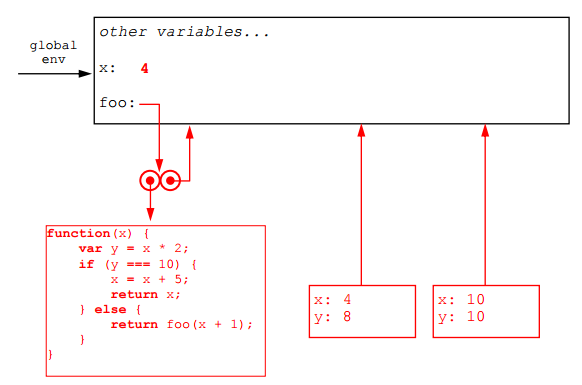
\includegraphics[width=1\linewidth]{screenshot003}
  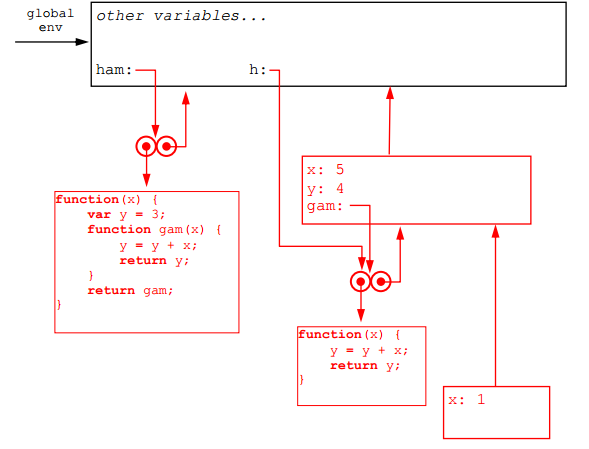
\includegraphics[width=1\linewidth]{screenshot004}

  \section{Contest Entries for "inspiration"}
   {\tiny jk, these are just paddings}\\
  
\includegraphics[width=0.49\linewidth]{screenshot006}\hfill
  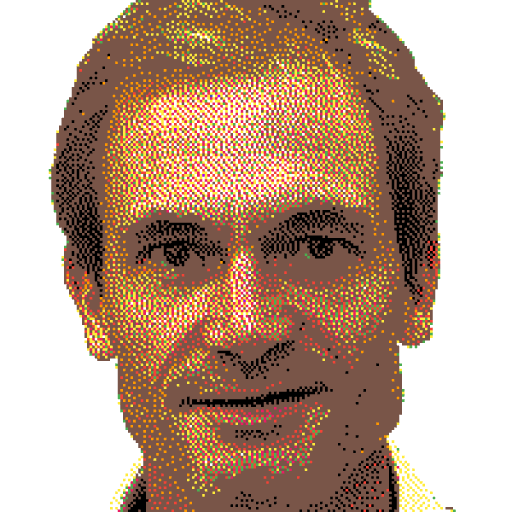
\includegraphics[width=0.49\linewidth]{screenshot005}

  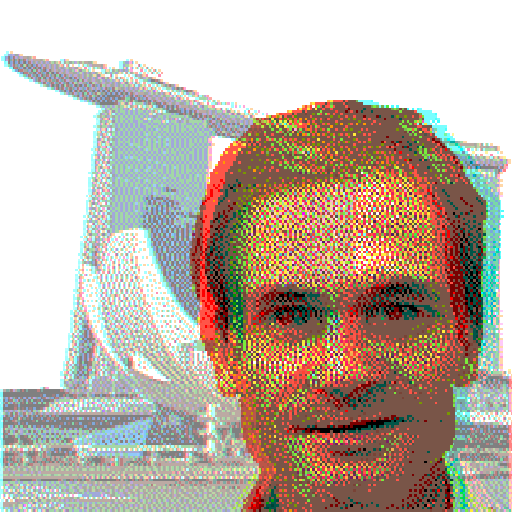
\includegraphics[width=0.49\linewidth]{screenshot007}\hfill
  
\includegraphics[width=0.49\linewidth]{screenshot008}

  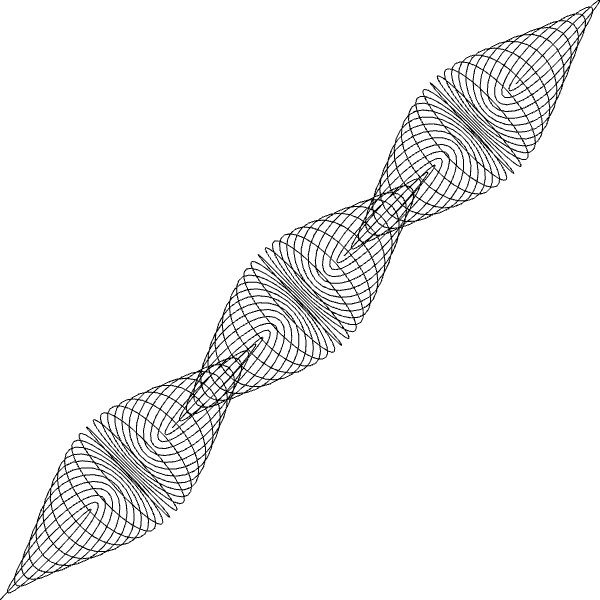
\includegraphics[width=1\linewidth]{screenshot009}

  \section{Dank Meme}
  
\includegraphics[width=1\linewidth]{screenshot010}

  \section{20th Anniversary, from IC1101S to CS1101S, from 1997 to 2017}
  Woah the module is as old as me!\\
  
\includegraphics[width=0.49\linewidth]{screenshot011}\hfill
  
\includegraphics[width=0.49\linewidth]{screenshot012}


  %   \begin{minted}{javascript}

  %   \end{minted}
\end{multicols*}
\end{document}
